\subsection{Chiffrement symétrique}

\begin{frame}{Chiffrement : définition}
  \begin{block}{Définition : chiffrement}
    Le chiffrement est une technique permettant à deux parties d'échanger de manière sécurisée.
    Il existe deux grands types de chiffrements, dits symétrique et asymétrique.

    Les principales caractéristiques du chiffrement sont :

    \begin{itemize}
      \item Confidentialité : protéger contre l'accès non autorisé, seules les personnes ayant la clé puissent déchiffrer et lire le message.
      \item Intégrité : détecter toute modification ou altération des données chiffrées. Si les données chiffrées sont altérées, le déchiffrement donnera un résultat incorrect ou une erreur.
      \item Efficacité : traiter rapidement les données, en particulier lorsqu'il s'agit de volumes importants.
      \item Sécurité : être résistants aux attaques cryptographiques, telles que les attaques par force brute, les attaques de collision, différentielles\dots
    \end{itemize}
  \end{block}
\end{frame}

\begin{frame}{Modèle de canal de communication}
  \begin{figure}
  \resizebox{\columnwidth}{!}{%
    \begin{tikzpicture}
      % Actors
      \node[label=Alice] (alice) at (0,0) {\includegraphics[height=4cm]{img/alice.png}};
      \node[label=Bob] (bob) at (24,0) {\includegraphics[height=4cm]{img/bob.png}};
      \node[label=Eve] (eve) at (12,-4) {\includegraphics[height=4cm]{img/eve.png}};

      % Canal
      \draw (4,0) ellipse (0.35 and 0.5);
      \draw (20,-0.5) arc (-90:90:0.5);
      \draw (4,0.5) -- ++(16,0);
      \draw (4,-0.5) -- ++(16,0);
      \node (label) at (12, 1) {Canal de communication non sécurisé};

      \draw[->] (eve.west) -- ++(-1.5,0) -- node[left] {Écoute} ++(0,3.5);
      \draw[->] (eve.east) -- ++(1.5,0) --  node[right] {Modifie} ++(0,3.5);

    \end{tikzpicture}%
  }

  \caption{Modèle de canal de communication non sécurisé}
\end{figure}
\end{frame}

\begin{frame}{Chiffrement symétrique}
  \begin{block}{Définition : chiffrement symétrique}
    Le chiffrement symétrique est une technique de chiffrement où \textbf{une seule et même clé} est utilisée à la fois pour le \textbf{chiffrement et le déchiffrement} des données.
    Cela signifie que l'émetteur et le destinataire du message doivent partager la même clé secrète pour pouvoir communiquer de manière sécurisée.

    \vspace{1em}

    Exemples d'algorithmes de chiffrement symétriques :

    \begin{itemize}
      \item AES
      \item DES (obslète) et triple DES
    \end{itemize}
  \end{block}
\end{frame}

\begin{frame}{Chiffrement symétrique : modèle}
  \begin{figure}
  \resizebox{\columnwidth}{!}{%
    \begin{tikzpicture}
      % Actors
      \node[label=Alice + clé $K$] (alice) at (0,0) {\includegraphics[height=4cm]{img/alice.png}};
      \node[label=Bob + clé $K$] (bob) at (24,0) {\includegraphics[height=4cm]{img/bob.png}};
      \node[label=Eve sans clé] (eve) at (12,-4) {\includegraphics[height=4cm]{img/eve.png}};

      \node[draw] (alice_clear) at (3,0) {Message};
      \node[draw] (cipher) at (12,0) {\#\&*YU*F};
      \node[draw] (bob_clear) at (21,0) {Message};

      \draw[->] (alice_clear.east) -- (cipher) node[near start,above,sloped]{Chiffre avec $K$};
      \draw[->] (cipher.east) -- (bob_clear) node[near end,above,sloped]{Déchiffre avec $K$};

      % Canal
      \draw (8,0) ellipse (0.35 and 0.5);
      \draw (16,-0.5) arc (-90:90:0.5);
      \draw (8,0.5) -- ++(8,0);
      \draw (8,-0.5) -- ++(8,0);
      \node (label) at (12, 1) {Canal de communication non sécurisé};

      \draw[->] (eve.west) -- ++(-1.5,0) -- node[left] {Écoute} ++(0,3.5);
      \draw[->] (eve.east) -- ++(1.5,0) --  node[right] {Modifie} ++(0,3.5);
    \end{tikzpicture}%
  }

  \caption{Chiffrement symétrique avec une clé $K$}
\end{figure}
\end{frame}

\begin{frame}{Chiffrement symétrique : exercice}
  \begin{block}{Exercice : échange d'information sur canal public}
    \begin{enumerate}
      \item Aller sur \url{https://www.devglan.com/online-tools/aes-encryption-decryption}
      \item Choisir une clé de 32 caractères hexadécimaux (par ex: \texttt{770A8A65DA156D24EE2A093277530142}).
      \item Partager la clé avec un ami.
      \item Chiffrer un message et le publier sur un canal public.
      \item Vérifier que l'ami est capable de déchiffrer le message et personne d'autre.
    \end{enumerate}
  \end{block}
\end{frame}

\begin{frame}{Chiffrement symétrique : résumé}
  \begin{itemize}
    \item Le chiffrement symétrique permet d'échanger des messages secrets.
    \item Une seule clé pour chiffrer et déchiffrer $\Rightarrow$ l'émetteur et le destinataire doivent connaître la clé.
    \item AES est l'algorithme le plus utilisé.
  \end{itemize}

  Problème : comment partager la clé de manière sécurisée ?
\end{frame}

\begin{frame}{Modes de chiffrement}
  \begin{columns}
    \begin{column}{0.6\textwidth}
      \begin{itemize}
        \item ECB (Electronic CodeBook)
          \begin{itemize}
            \item Le plus simple mais le moins sécurisé
            \item Motifs visibles dans les données chiffrées
          \end{itemize}
        \item CBC (Cipher Block Chaining)
          \begin{itemize}
            \item Utilise un vecteur d'initialisation (IV)
            \item Chaque bloc dépend du précédent
          \end{itemize}
        \item CTR (Counter)
          \begin{itemize}
            \item Transforme le chiffrement par bloc en flux
            \item Parallélisable
          \end{itemize}
        \item GCM (Galois/Counter Mode)
          \begin{itemize}
            \item Authentification intégrée
            \item Recommandé pour TLS
          \end{itemize}
      \end{itemize}
    \end{column}
    \begin{column}{0.4\textwidth}
      \begin{center}
        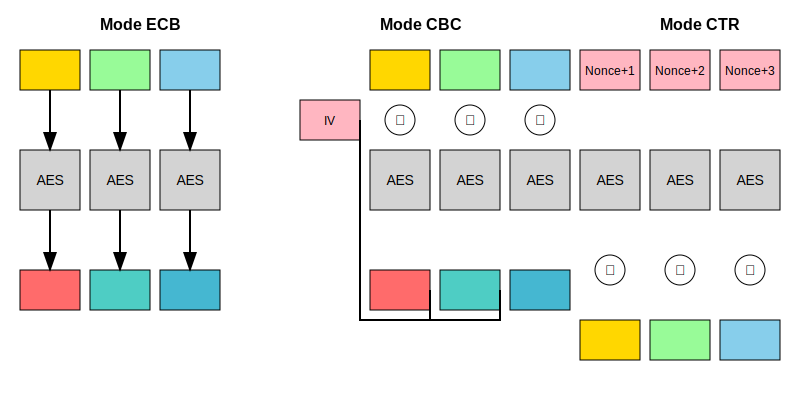
\includegraphics[width=\textwidth]{img/encryption-modes.png}
      \end{center}
    \end{column}
  \end{columns}
\end{frame}

\begin{frame}[fragile]{Exemple pratique avec Node.js}
  \begin{minted}[fontsize=\scriptsize]{javascript}
    const crypto = require('crypto');

    // Génération de la clé et du vecteur d'initialisation
    const key = crypto.randomBytes(32); // 256 bits pour AES-256
    const iv = crypto.randomBytes(16);  // 128 bits pour AES

    // Chiffrement
    function encrypt(text) {
      const cipher = crypto.createCipheriv(
        'aes-256-cbc', key, iv
      );
      let encrypted = cipher.update(text, 'utf8', 'hex');
      encrypted += cipher.final('hex');
      return encrypted;
    }

    // Déchiffrement
    function decrypt(encrypted) {
      const decipher = crypto.createDecipheriv(
        'aes-256-cbc', key, iv
      );
      let decrypted = decipher.update(encrypted, 'hex', 'utf8');
      decrypted += decipher.final('utf8');
      return decrypted;
    }

    const message = "Message secret";
    const encrypted = encrypt(message);
    console.log("Chiffré:", encrypted);
    console.log("Déchiffré:", decrypt(encrypted));
  \end{minted}

  \begin{itemize}
    \item Utilise AES-256 en mode CBC
    \item Gestion explicite de la clé et de l'IV
    \item Format hexadécimal pour le texte chiffré
  \end{itemize}
\end{frame}

\begin{frame}{Applications courantes}
  \begin{itemize}
    \item Chiffrement de disque
      \begin{itemize}
        \item BitLocker (Windows)
        \item FileVault (macOS)
        \item LUKS (Linux)
      \end{itemize}
    \item Communications sécurisées
      \begin{itemize}
        \item WiFi (WPA3)
        \item VPN
        \item Session TLS
      \end{itemize}
    \item Stockage cloud
      \begin{itemize}
        \item Chiffrement côté client
        \item Chiffrement au repos
      \end{itemize}
  \end{itemize}
\end{frame}

\begin{frame}{Performance et sécurité}
  \begin{columns}
    \begin{column}{0.5\textwidth}
      Tailles de clé courantes :
      \begin{itemize}
        \item AES-128 : 128 bits
        \item AES-192 : 192 bits
        \item AES-256 : 256 bits
      \end{itemize}

      Performances :
      \begin{itemize}
        \item Instructions AES-NI
        \item \textasciitilde 1 Go/s sur CPU moderne
        \item Adapté au chiffrement temps réel
      \end{itemize}
    \end{column}

    \begin{column}{0.5\textwidth}
      Bonnes pratiques :
      \begin{itemize}
        \item Rotation régulière des clés
        \item Stockage sécurisé des clés
        \item Utilisation de sel (IV)
        \item Mode authentifié (GCM)
      \end{itemize}
    \end{column}
  \end{columns}
\end{frame}